\section{Serial\-Handler Class Reference}
\label{classSerialHandler}\index{SerialHandler@{SerialHandler}}
{\tt \#include $<$Serial\-Handler.h$>$}

Inheritance diagram for Serial\-Handler::\begin{figure}[H]
\begin{center}
\leavevmode
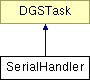
\includegraphics[height=2cm]{classSerialHandler}
\end{center}
\end{figure}
\subsection*{Public Member Functions}
\begin{CompactItemize}
\item 
{\bf Serial\-Handler} (void)
\item 
{\bf $\sim$Serial\-Handler} (void)
\item 
int {\bf initialize} (void)
\item 
virtual int {\bf svc} ()
\end{CompactItemize}
\subsection*{Protected Member Functions}
\begin{CompactItemize}
\item 
virtual void {\bf handle\_\-read\_\-stream} (const ACE\_\-Asynch\_\-Read\_\-Stream::Result \&result)
\item 
virtual void {\bf handle\_\-write\_\-stream} (const ACE\_\-Asynch\_\-Write\_\-Stream::Result \&result)
\end{CompactItemize}


\subsection{Detailed Description}
Implements the Serial Adaptor 



\subsection{Constructor \& Destructor Documentation}
\index{SerialHandler@{Serial\-Handler}!SerialHandler@{SerialHandler}}
\index{SerialHandler@{SerialHandler}!SerialHandler@{Serial\-Handler}}
\subsubsection{\setlength{\rightskip}{0pt plus 5cm}Serial\-Handler::Serial\-Handler (void)}\label{classSerialHandler_a0}


{\bf Serial\-Handler::Serial\-Handler}{\rm (p.\,\pageref{classSerialHandler_a0})} \index{SerialHandler@{Serial\-Handler}!~SerialHandler@{$\sim$SerialHandler}}
\index{~SerialHandler@{$\sim$SerialHandler}!SerialHandler@{Serial\-Handler}}
\subsubsection{\setlength{\rightskip}{0pt plus 5cm}Serial\-Handler::$\sim${\bf Serial\-Handler} (void)}\label{classSerialHandler_a1}


{\bf Serial\-Handler::$\sim$Serial\-Handler}{\rm (p.\,\pageref{classSerialHandler_a1})} Destructor. 

\begin{Desc}
\item[{\bf Todo}]close correctly all the streams \end{Desc}


\subsection{Member Function Documentation}
\index{SerialHandler@{Serial\-Handler}!handle_read_stream@{handle\_\-read\_\-stream}}
\index{handle_read_stream@{handle\_\-read\_\-stream}!SerialHandler@{Serial\-Handler}}
\subsubsection{\setlength{\rightskip}{0pt plus 5cm}void Serial\-Handler::handle\_\-read\_\-stream (const ACE\_\-Asynch\_\-Read\_\-Stream::Result \& {\em result})\hspace{0.3cm}{\tt  [protected, virtual]}}\label{classSerialHandler_b0}


handle\_\-read\_\-stream

\begin{Desc}
\item[Parameters:]
\begin{description}
\item[{\em result}]\end{description}
\end{Desc}


\begin{Desc}
\item[{\bf Todo}]Chech if the compartion can be done in a more eficient way \end{Desc}
\index{SerialHandler@{Serial\-Handler}!handle_write_stream@{handle\_\-write\_\-stream}}
\index{handle_write_stream@{handle\_\-write\_\-stream}!SerialHandler@{Serial\-Handler}}
\subsubsection{\setlength{\rightskip}{0pt plus 5cm}void Serial\-Handler::handle\_\-write\_\-stream (const ACE\_\-Asynch\_\-Write\_\-Stream::Result \& {\em result})\hspace{0.3cm}{\tt  [protected, virtual]}}\label{classSerialHandler_b1}


handle\_\-write\_\-stream

\begin{Desc}
\item[Parameters:]
\begin{description}
\item[{\em result}]\end{description}
\end{Desc}
\index{SerialHandler@{Serial\-Handler}!initialize@{initialize}}
\index{initialize@{initialize}!SerialHandler@{Serial\-Handler}}
\subsubsection{\setlength{\rightskip}{0pt plus 5cm}int Serial\-Handler::initialize (void)}\label{classSerialHandler_a2}


initialize starts the inizialization of the serial device and attach it to the reading streams.

\begin{Desc}
\item[Returns:]\end{Desc}
\index{SerialHandler@{Serial\-Handler}!svc@{svc}}
\index{svc@{svc}!SerialHandler@{Serial\-Handler}}
\subsubsection{\setlength{\rightskip}{0pt plus 5cm}int Serial\-Handler::svc ()\hspace{0.3cm}{\tt  [virtual]}}\label{classSerialHandler_a3}


svc This is the internal loop of the ACETask, it read from the standart input.

\begin{Desc}
\item[Returns:]\end{Desc}


The documentation for this class was generated from the following files:\begin{CompactItemize}
\item 
{\bf Serial\-Handler.h}\item 
{\bf Serial\-Handler.cpp}\end{CompactItemize}
